\chapter{被子植物的有性生殖}\label{ch:b2:angiosperm-reproduction}

五月的苹果园，花开一片白，蜜蜂嗡嗡作响；
十月，同一批树上\omterm{def:b2:angiosperm-reproduction:seed}{果实}累累，每个苹果
含十粒\omterm{def:b2:angiosperm-reproduction:seed}{种子}，每粒\omterm{def:b2:angiosperm-reproduction:seed}{种子}都是包裹着贮藏食物的胚态小树。
这一整个转变——花、由昆虫携带的\omterm{def:b2:plant-life-cycles:heterospory}{花粉}、
穿过花柱生长的\omterm{thm:b2:angiosperm-reproduction:tube}{花粉管}、\omterm{prop:b2:angiosperm-reproduction:double}{双
受精}（同时形成胚和\omterm{prop:b2:angiosperm-reproduction:double}{胚乳}营养供应）、
\omterm{def:b2:angiosperm-reproduction:flower}{子房}膨大成供食用的\omterm{def:b2:angiosperm-reproduction:seed}{果实}——正是这一发明，
在约一亿年间使被子植物成为
陆地上占优势的植物。本章从花讲到
扩散的\omterm{def:b2:angiosperm-reproduction:seed}{种子}。

\section{花}

\begin{definition}[花的组成]\label{def:b2:angiosperm-reproduction:flower}
\index{花}\index{雄蕊}\index{心皮}\index{子房}\index{柱头}
\emph{花}是一种短枝，其叶片转化为
四轮。外侧的\emph{萼片}（合称花萼）保护
花蕾；然后是\emph{花瓣}（即花冠），起招引\omterm{def:b2:angiosperm-reproduction:pollination}{传粉}者的作用；然后是
\emph{雄蕊}，每枚由花丝和顶端的\emph{花药}构成，
花药含四个\omterm{def:b2:plant-life-cycles:heterospory}{花粉}囊；花的中央则是一枚或多枚\emph{心皮}，
每枚心皮折叠闭合，形成\emph{雌蕊}，其上有可接受\omterm{def:b2:plant-life-cycles:heterospory}{花粉}的
\emph{柱头}、\emph{花柱}和\emph{子房}，子房内包藏
\emph{\omterm{def:b2:plant-life-cycles:heterospory}{胚珠}}。兼有雄蕊和心皮的花为
\emph{雌雄同体}（多数物种）；\emph{雌雄同株}的植物
在同一个体上着生分开的雄花和雌花（玉米、栎、
榛），\emph{雌雄异株}的物种则是雄花和雌花分生于不同个体上（冬青、
柳、海枣）。封闭心皮——即被子植物得名的
特征——的意义在于\omterm{def:b2:plant-life-cycles:heterospory}{胚珠}被包藏：
\omterm{def:b2:plant-life-cycles:heterospory}{花粉}不能直接抵达\omterm{def:b2:plant-life-cycles:heterospory}{胚珠}，而必须沿植物组织
生长至\omterm{def:b2:plant-life-cycles:heterospory}{胚珠}处，这使植物得以进行选择。
\end{definition}

\begin{omfigure}
\begin{tikzpicture}[every node/.style={font=\scriptsize}]
  % receptacle and pedicel
  \draw[thick] (0,-2.6) -- (0,-1.6);
  \draw[thick, fill=omExo!20] (-0.9,-1.6) .. controls (-1.0,-1.0) and (1.0,-1.0) .. (0.9,-1.6) -- cycle;
  % sepals
  \foreach \s in {-1,1} \draw[thick, fill=omExo!45] (0.6*\s,-1.4) .. controls (2.0*\s,-1.2) and (2.6*\s,-0.2) .. (2.8*\s,0.6) .. controls (2.0*\s,0.2) and (1.2*\s,-0.6) .. (0.6*\s,-1.4);
  % petals
  \foreach \s in {-1,1} \draw[thick, fill=omThm!15] (0.5*\s,-1.2) .. controls (1.6*\s,0.4) and (2.2*\s,1.8) .. (1.6*\s,3.0) .. controls (1.0*\s,2.0) and (0.5*\s,0.8) .. (0.5*\s,-1.2);
  % ovary with ovules
  \draw[thick, fill=omDef!12] (0,-0.7) ellipse (0.55 and 0.75);
  \foreach \p in {(-0.22,-0.5),(-0.22,-0.9),(0.22,-0.5),(0.22,-0.9)} \draw[thick, omDef, fill=omDef!40] \p circle (0.11);
  % style and stigma
  \draw[thick, fill=omDef!12] (-0.1,0.05) rectangle (0.1,1.9);
  \draw[thick, fill=omDef!40] (0,2.0) ellipse (0.28 and 0.14);
  % stamens
  \foreach \s in {-1,1} { \draw[thick] (0.35*\s,-1.0) .. controls (0.6*\s,0.2) .. (0.9*\s,1.5); \draw[thick, fill=omProp!60] (0.9*\s,1.6) ellipse (0.14 and 0.32); }
  % labels: right side
  \draw (0.28,2.0) -- (3.2,2.6) node[right] {柱头};
  \draw (0.1,1.2) -- (3.2,1.9) node[right] {花柱};
  \draw (0.55,-0.6) -- (3.2,1.2) node[right] {子房};
  \draw (0.22,-0.9) -- (3.2,0.5) node[right] {胚珠};
  \draw (2.6,0.35) -- (3.2,-0.4) node[right] {萼片};
  % labels: left side
  \draw (-1.5,2.4) -- (-2.6,2.8) node[left] {花瓣};
  \draw (-0.95,1.9) -- (-2.6,1.9) node[left] {花药};
  \draw (-0.65,0.6) -- (-2.6,0.9) node[left] {花丝};
  \draw (0,-2.2) -- (-2.6,-2.2) node[left] {花托和花梗};
  \node[anchor=west, align=left] at (5.4,0.5) {柱头 + 花柱 + 子房 \\$=$ 心皮（雌蕊）};
  \node[anchor=west, align=left] at (5.4,-0.8) {花药 + 花丝 \\$=$ 雄蕊};
\end{tikzpicture}

{\small 花的纵切面：萼片、花瓣、\omterm{def:b2:angiosperm-reproduction:flower}{雄蕊}
（花丝和花药）以及位于中央的\omterm{def:b2:angiosperm-reproduction:flower}{心皮}——\omterm{def:b2:angiosperm-reproduction:flower}{柱头}、
花柱和\omterm{def:b2:angiosperm-reproduction:flower}{子房}——包藏着\omterm{def:b2:plant-life-cycles:heterospory}{胚珠}。}
\end{omfigure}

\begin{omfigure}
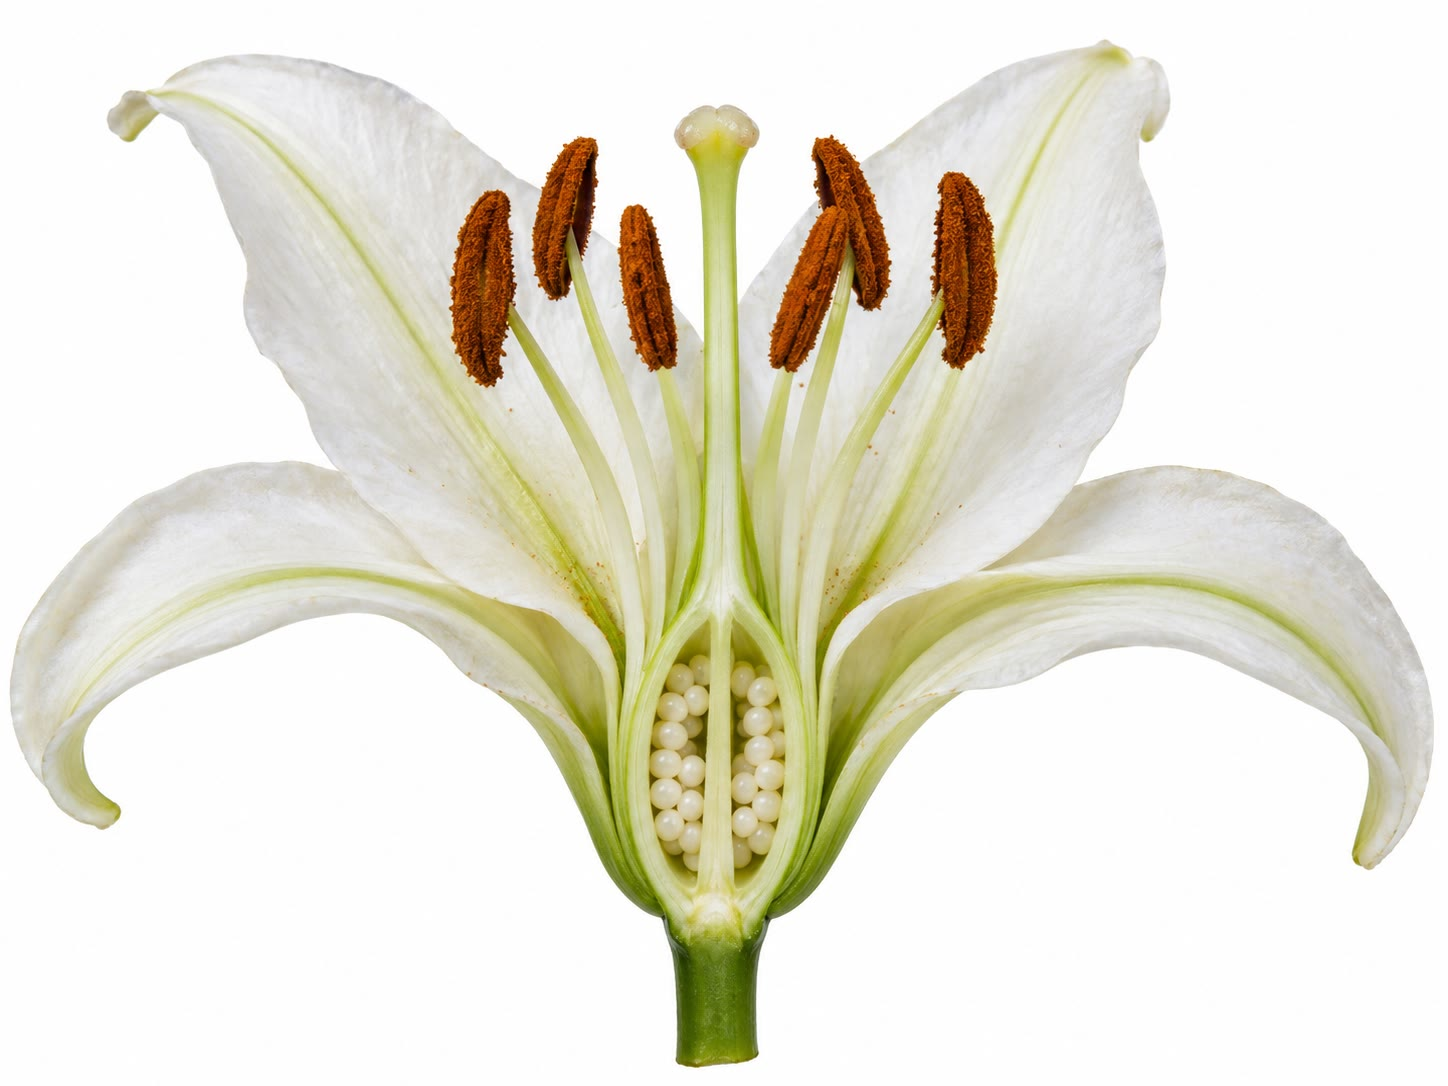
\includegraphics[width=0.55\linewidth]{images/book4/ai/b4-06-lily-dissected.jpg}

{\small 百合纵切：六枚\omterm{def:b2:angiosperm-reproduction:flower}{雄蕊}带着满是\omterm{def:b2:plant-life-cycles:heterospory}{花粉}的
花药，长花柱及其黏性\omterm{def:b2:angiosperm-reproduction:flower}{柱头}，以及打开的\omterm{def:b2:angiosperm-reproduction:flower}{子房}，
显示其中排列的\omterm{def:b2:plant-life-cycles:heterospory}{胚珠}。}
\end{omfigure}

\section{两种配子体}

\begin{proposition}[花粉：雄配子体]\label{prop:b2:angiosperm-reproduction:pollen}
\index{花粉粒}\index{小孢子发生}\index{孢粉素}
每个\omterm{def:b2:plant-life-cycles:heterospory}{花粉}囊中，\omterm{def:b2:meiosis-heredity:meiosis}{二倍体}的\omterm{def:b2:plant-life-cycles:heterospory}{花粉}母细胞经\omterm{def:b2:meiosis-heredity:meiosis}{减数分裂}产生
四分体，即\emph{\omterm{def:b2:plant-life-cycles:heterospory}{小孢子}}。每个\omterm{def:b2:plant-life-cycles:heterospory}{小孢子}经一次
不均等分裂，形成大的\emph{营养细胞}和小的
被包裹于其内的\emph{生殖细胞}；生殖细胞
再分裂一次（可在授粉前或授粉后），形成两个
\emph{精子}。成熟的\emph{\omterm{prop:b2:angiosperm-reproduction:pollen}{花粉粒}}因此是
一个三细胞的\omterm{def:b2:meiosis-heredity:meiosis}{单倍体}生物体——即整个雄\omterm{def:b2:plant-life-cycles:cycles}{配子体}——
大小为\qtyrange{10}{100}{\micro m}，外壁由
其外层为\emph{\omterm{prop:b2:angiosperm-reproduction:pollen}{孢粉素}}的壁包被，\omterm{prop:b2:angiosperm-reproduction:pollen}{孢粉素}是已知最耐受的生物聚合物，
壁面雕刻有该物种特有的刺、孔和沟纹，
这正是\omterm{def:b2:plant-life-cycles:heterospory}{花粉}能在沉积物中鉴定植物的原因，即使沉积物已有
数千万年之久。\omterm{prop:b2:angiosperm-reproduction:pollen}{花粉粒}以脱水状态散出，可存活
数小时（禾本科植物）至数周（某些树木），直到抵达\omterm{def:b2:angiosperm-reproduction:flower}{柱头}。
\end{proposition}

\begin{omfigure}
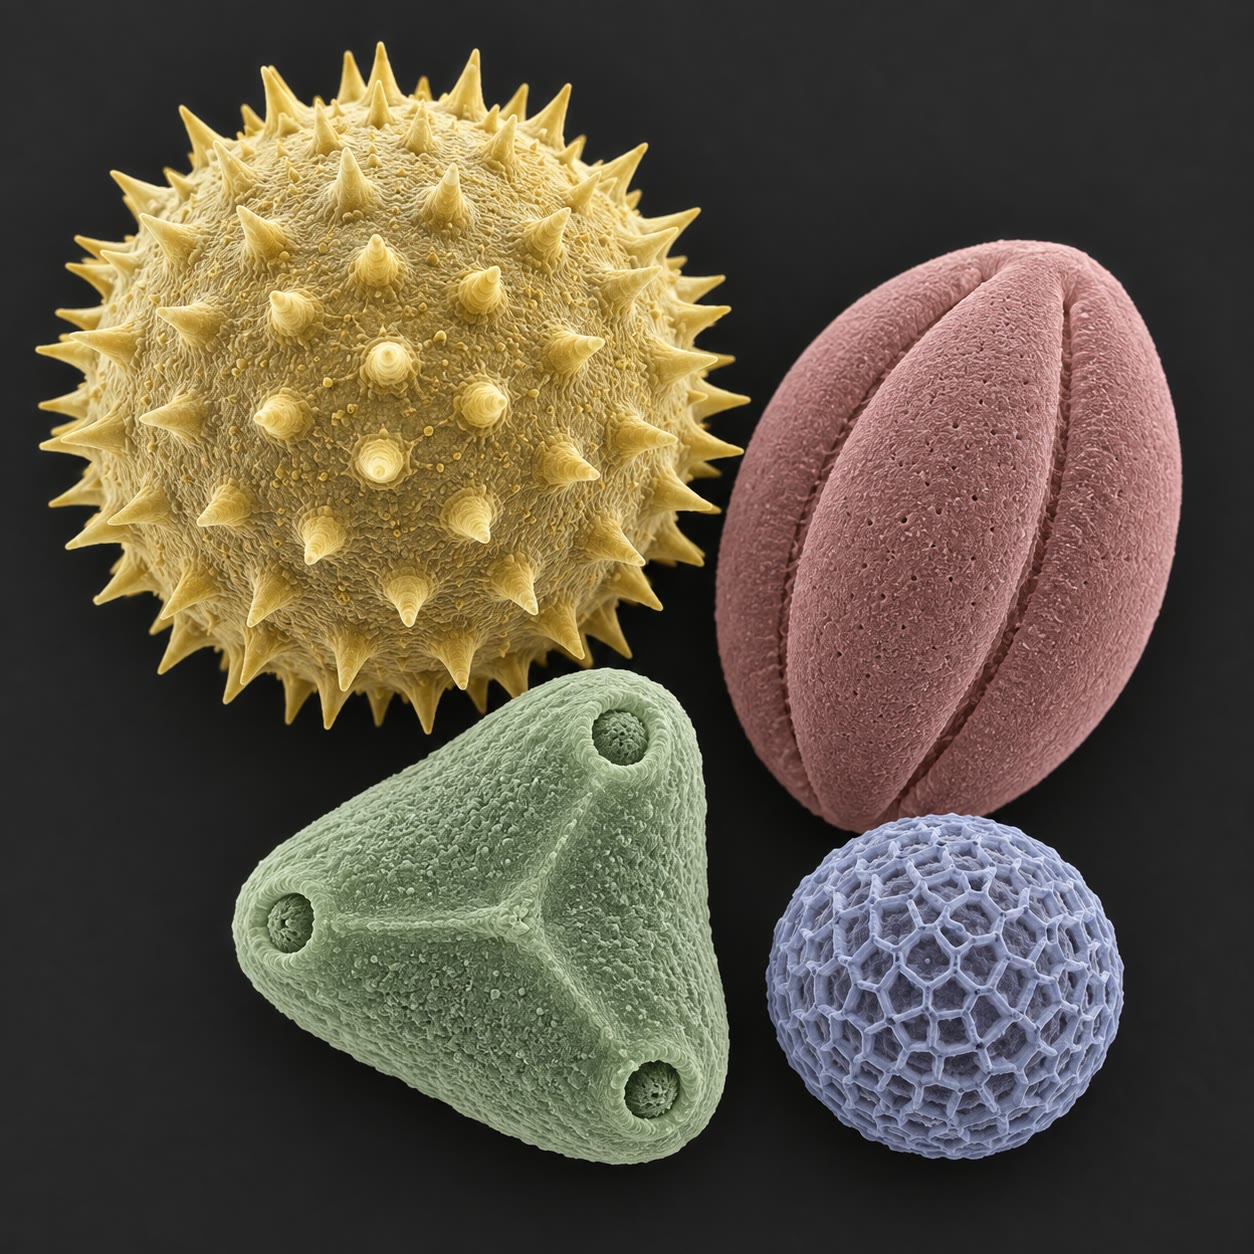
\includegraphics[width=0.45\linewidth]{images/book4/ai/b4-06-pollen-sem.jpg}

{\small 扫描电子显微镜下的\omterm{prop:b2:angiosperm-reproduction:pollen}{花粉粒}：每个物种的
\omterm{prop:b2:angiosperm-reproduction:pollen}{孢粉素}壁都有其独特的纹饰——刺、
沟纹、孔、网状结构——据此可以识别该物种。}
\end{omfigure}

\begin{proposition}[胚囊：雌配子体]\label{prop:b2:angiosperm-reproduction:embryosac}
\index{胚囊}\index{大孢子发生}\index{极核}
每个\omterm{def:b2:plant-life-cycles:heterospory}{胚珠}中，珠心内的一个\omterm{def:b2:meiosis-heredity:meiosis}{二倍体}细胞经\omterm{def:b2:meiosis-heredity:meiosis}{减数分裂}，
四个\omterm{def:b2:plant-life-cycles:heterospory}{大孢子}中有三个退化，剩下的一个通过
三次有丝分裂（核分裂而细胞不分裂），发育成一个八核、
七细胞的\emph{\omterm{prop:b2:angiosperm-reproduction:embryosac}{胚囊}}：珠孔端为\emph{卵细胞}，
两侧各有两个\emph{助细胞}；另一端为三个
\emph{反足细胞}；中央为一个大的\emph{中央细胞}，
其中含两个\emph{\omterm{prop:b2:angiosperm-reproduction:embryosac}{极核}}。这个\omterm{prop:b2:angiosperm-reproduction:embryosac}{胚囊}被珠心和
带有珠孔的两层珠被包裹，即整个雌\omterm{def:b2:plant-life-cycles:cycles}{配子体}——
七个细胞，相当于\omterm{def:b2:plant-life-cycles:moss}{苔藓}的整株植物。两个\omterm{prop:b2:angiosperm-reproduction:embryosac}{极核}
与卵细胞在遗传上完全相同，这一事实对
\omterm{prop:b2:angiosperm-reproduction:double}{胚乳}而言至关重要。
\end{proposition}

\begin{omfigure}
\begin{tikzpicture}[every node/.style={font=\scriptsize}]
  % pollen grain
  \begin{scope}
    \draw[very thick, omProp!80!black, fill=omProp!15] (0,0) circle (1.1);
    \draw[thick, omProp!80!black] (0,0) circle (0.95);
    \foreach \a in {0,30,...,330} \draw[omProp!80!black, thick] (\a:1.1) -- (\a:1.25);
    \draw[thick, fill=omDef!25] (0.15,-0.2) ellipse (0.55 and 0.4); \node[font=\tiny] at (0.15,-0.2) {营养细胞};
    \draw[thick, fill=omThm!30] (-0.3,0.45) ellipse (0.22 and 0.14); \draw[thick, fill=omThm!30] (0.2,0.5) ellipse (0.22 and 0.14);
    \draw[omThm] (0.0,0.62) -- (0.0,1.5); \node[omThm, anchor=south] at (0.0,1.5) {两个精子};
    \node[below, align=center] at (0,-1.4) {花粉粒（$n$）\\3 个细胞，孢粉素壁};
  \end{scope}
  % ovule with embryo sac
  \begin{scope}[xshift=5.5cm]
    \draw[thick, fill=omExo!25] (0,0) ellipse (1.5 and 2.1);
    \draw[thick, fill=omExo!10] (0,0) ellipse (1.15 and 1.75);
    \fill[white] (-0.3,1.7) rectangle (0.3,2.2); \draw[thick] (-0.3,1.7) -- (-0.3,2.15); \draw[thick] (0.3,1.7) -- (0.3,2.15);
    \draw[thick, fill=white] (0,0) ellipse (0.7 and 1.35);
    % cells: egg + synergids top, central, antipodals bottom
    \draw[thick, fill=omThm!30] (0,0.95) circle (0.17); \node[omThm, anchor=west] at (1.6,1.2) {卵细胞};
    \draw[thick, fill=omDef!25] (-0.35,1.0) circle (0.14); \draw[thick, fill=omDef!25] (0.35,1.0) circle (0.14); \node[anchor=west] at (1.6,0.75) {两个助细胞};
    \draw[thick, fill=omDef!10] (0,0) ellipse (0.55 and 0.6); \fill[omDef!80!black] (-0.15,0.05) circle (0.09); \fill[omDef!80!black] (0.15,0.05) circle (0.09);
    \node[anchor=west, align=left] at (1.6,0.1) {中央细胞，\\含两个极核};
    \foreach \x in {-0.3,0,0.3} \draw[thick, fill=omDef!25] (\x,-1.0) circle (0.13); \node[anchor=west] at (1.6,-1.0) {三个反足细胞};
    \draw (0.35,2.0) -- (1.6,2.0) node[right] {珠孔};
    \draw (1.3,-0.9) -- (1.6,-1.6) node[right] {珠被};
    \draw (0.9,-1.35) -- (1.6,-2.1) node[right] {珠心};
    \draw (1.6,1.2) -- (0.17,0.95); \draw (1.6,0.75) -- (0.49,1.0); \draw (1.6,0.1) -- (0.55,0.05); \draw (1.6,-1.0) -- (0.43,-1.0);
    \node[below, align=center] at (0,-2.3) {带胚囊的胚珠（$n$）\\7 个细胞，8 个核};
  \end{scope}
\end{tikzpicture}

{\small 被子植物的两种\omterm{def:b2:plant-life-cycles:cycles}{配子体}，均已退化为
仅含少数细胞：三细胞的\omterm{prop:b2:angiosperm-reproduction:pollen}{花粉粒}，以及
\omterm{def:b2:plant-life-cycles:heterospory}{胚珠}内七细胞的\omterm{prop:b2:angiosperm-reproduction:embryosac}{胚囊}。}
\end{omfigure}

\section{传粉}

\begin{definition}[传粉及其媒介]\label{def:b2:angiosperm-reproduction:pollination}
\index{传粉}\index{传粉综合征}\index{花蜜}
\emph{传粉}是\omterm{def:b2:plant-life-cycles:heterospory}{花粉}从花药转移到
\omterm{def:b2:angiosperm-reproduction:flower}{柱头}；\emph{自花传粉}指同一朵花或同一植株内的传粉，
\emph{异花传粉}指植株之间的传粉。\emph{风媒}花（禾草、橡树、桦树、车前）
体型小、颜色绿，
无香味，\omterm{def:b2:angiosperm-reproduction:flower}{柱头}大而呈羽毛状，\omterm{def:b2:plant-life-cycles:heterospory}{花粉}数量极多，
\omterm{def:b2:plant-life-cycles:heterospory}{花粉}光滑干燥；\omterm{def:b2:plant-life-cycles:heterospory}{花粉}与\omterm{def:b2:plant-life-cycles:heterospory}{胚珠}之比高达百万。
\emph{动物媒}花以回报传粉者：\emph{花蜜}
（蜜腺分泌的糖溶液）、\omterm{def:b2:plant-life-cycles:heterospory}{花粉}本身、油脂、香气；
并以颜色、形状和气味“做广告”，且与传粉者的感觉相匹配——
例如供蜜蜂识别的紫外线蜜导（蜜蜂能见紫外线而不见红色）；
无香味的红色管状花供蜂鸟采食；
白色、香味浓烈、夜间开放、花管深长的花供蛾类传粉；
褐色、有恶臭的花供食腐蝇传粉；
粗壮、色淡的夜花供蝙蝠传粉。每一组这样的性状构成一个\emph{传粉
综合征}，而花与传粉者之间的契合，是
\emph{协同演化}的教科书式范例：达尔文根据一种马达加斯加兰花的
\qty{30}{cm}长的蜜距，预言存在一种口器长
\qty{30}{cm}的蛾，四十年后果然被发现。
\end{definition}

\begin{omfigure}
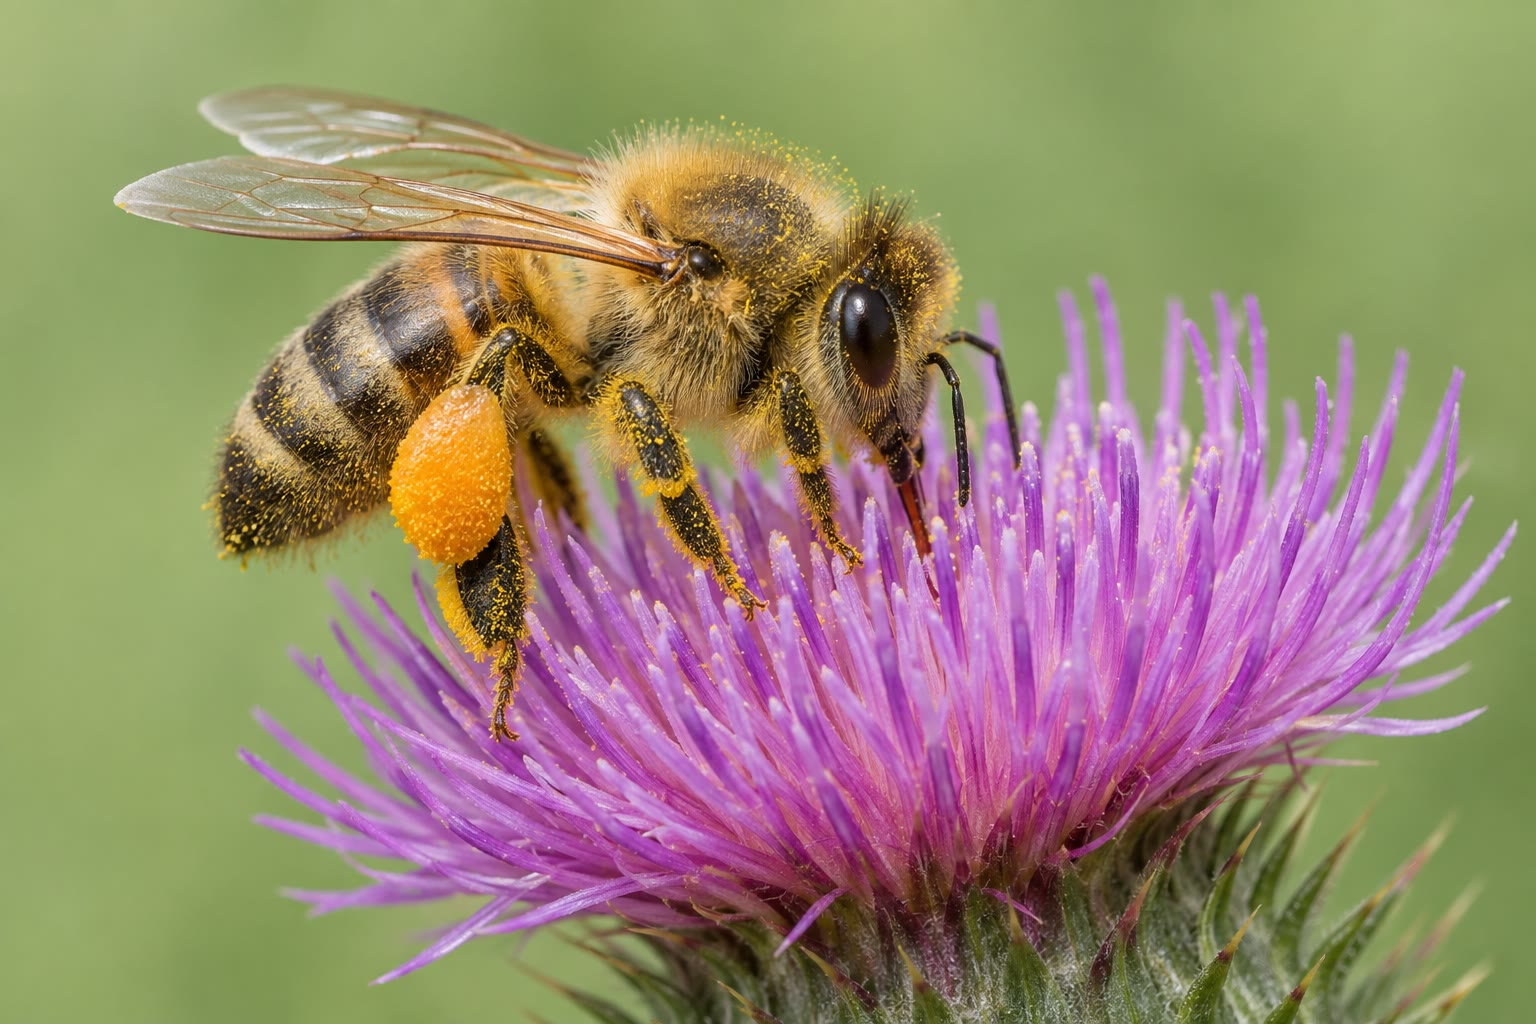
\includegraphics[width=0.58\linewidth]{images/book4/ai/b4-06-bee-on-flower.jpg}

{\small 一只停在蓟花上的蜜蜂：\omterm{def:b2:plant-life-cycles:heterospory}{花粉}沾满其身体，并填入后腿的
\omterm{def:b2:plant-life-cycles:heterospory}{花粉}篮；其中一部分会落到它随后访问的另一朵蓟花的\omterm{def:b2:angiosperm-reproduction:flower}{柱头}上。
紫色、可供着陆的平台和丰富的\omterm{def:b2:angiosperm-reproduction:pollination}{花蜜}，
均为蜜蜂\omterm{def:b2:angiosperm-reproduction:pollination}{传粉综合征}的特征。}
\end{omfigure}

\begin{proposition}[避免自花受精]\label{prop:b2:angiosperm-reproduction:selfing}
\index{自交不亲和}\index{花柱异型}\index{雌雄异熟}
雌雄同花可以自花受精，许多植物确实如此（豌豆、
小麦、番茄）；但自交会暴露\omterm{def:b2:meiosis-heredity:vocabulary}{隐性}有害\omterm{def:b2:meiosis-heredity:vocabulary}{等位基因}，
（\emph{近交衰退}），因此多数物种会阻止自交。在时间上：
\emph{\omterm{prop:b2:angiosperm-reproduction:selfing}{雌雄异熟}}，花药与\omterm{def:b2:angiosperm-reproduction:flower}{柱头}成熟的时间不同
（伞形科和菊科多为\omterm{def:b2:angiosperm-reproduction:flower}{雄蕊}先熟）。在空间上：
\emph{雌雄异位}，花药与\omterm{def:b2:angiosperm-reproduction:flower}{柱头}彼此分开，如
报春花的\emph{\omterm{prop:b2:angiosperm-reproduction:selfing}{花柱异型}}，其中长柱花（花柱长、花药低）
与短柱花（花柱短、花药高）把\omterm{def:b2:plant-life-cycles:heterospory}{花粉}放在昆虫身上的不同部位；
从生化角度看：
\emph{\omterm{prop:b2:angiosperm-reproduction:selfing}{自交不亲和}}是一种识别系统：
携带与雌蕊共有的 $S$ \omterm{def:b2:meiosis-heredity:vocabulary}{等位基因}的\omterm{def:b2:plant-life-cycles:heterospory}{花粉}被拒绝。
在\emph{\omterm{def:b2:plant-life-cycles:cycles}{配子体}型}不亲和中（苹果、樱桃、矮牵牛、
禾草）由\omterm{def:b2:plant-life-cycles:heterospory}{花粉}本身的\omterm{def:b2:meiosis-heredity:meiosis}{单倍体} $S$ \omterm{def:b2:meiosis-heredity:vocabulary}{等位基因}决定：一个
$S_1S_2$ 的雌蕊在花柱中阻止 $S_1$ 与 $S_2$ 的\omterm{thm:b2:angiosperm-reproduction:tube}{花粉管}，故来自
$S_1S_3$ 植株的\omterm{def:b2:plant-life-cycles:heterospory}{花粉}一半可亲和，来自 $S_3S_4$ 植株的则全部可亲和。
在\emph{\omterm{def:b2:plant-life-cycles:cycles}{孢子体}型}不亲和（甘蓝、向日葵）中，
由\omterm{def:b2:plant-life-cycles:heterospory}{花粉}亲本的\omterm{def:b2:meiosis-heredity:meiosis}{二倍体}\omterm{def:b2:meiosis-heredity:vocabulary}{基因型}决定，作用发生在\omterm{def:b2:angiosperm-reproduction:flower}{柱头}表面。
稀有的 $S$ \omterm{def:b2:meiosis-heredity:vocabulary}{等位基因}几乎与所有其他个体可亲和，
因此选择使一个种群中保留了数十种\omterm{def:b2:meiosis-heredity:vocabulary}{等位基因}。
\end{proposition}
\begin{proof}[证据]
达尔文（1862，1877）以手工方式杂交报春花：来自短柱花的\omterm{def:b2:plant-life-cycles:heterospory}{花粉}
授于长柱花的\omterm{def:b2:angiosperm-reproduction:flower}{柱头}（“亲和”杂交）上，结出饱满的蒴果；
长柱花授长柱花或短柱花授短柱花（“不亲和”）时，结实很少，
甚至完全不结实，尽管植株健康、\omterm{def:b2:plant-life-cycles:heterospory}{花粉}也有活力。
达尔文断定两种花型彼此适应以便异交，并防止自花受精；
他还统计了数千次杂交中每个蒴果的\omterm{def:b2:angiosperm-reproduction:seed}{种子}数，
由此测定了数十个物种自花受精的代价：
自交后代更矮、更轻、可育性更低，
而且逐代如此。
\end{proof}

\begin{omfigure}
\begin{tikzpicture}[every node/.style={font=\scriptsize}]
  % pistil S1S2 with pollen tubes
  \draw[thick, fill=omDef!10] (-0.5,0) rectangle (0.5,3.2);
  \draw[thick, fill=omDef!30] (0,3.3) ellipse (0.7 and 0.2);
  \draw[thick, fill=omDef!12] (0,-0.6) ellipse (0.9 and 0.7);
  \node at (0,-0.6) {子房};
  \node[anchor=east] at (-1.1,3.3) {$S_1S_2$ 植株的柱头};
  % pollen grains
  \draw[thick, fill=omThm!40] (-0.35,3.75) circle (0.13); \node[omThm, left] at (-0.5,3.75) {$S_1$};
  \draw[thick, fill=omThm!40] (0,3.75) circle (0.13); \node[omThm, anchor=south] at (0,3.92) {$S_2$};
  \draw[thick, fill=omExo!70!black] (0.35,3.75) circle (0.13); \node[right] at (0.5,3.75) {$S_3$};
  % tubes: S1 and S2 stop in the style, S3 reaches the ovary
  \draw[thick, omThm] (-0.35,3.3) -- (-0.35,2.3); \node[omThm, left, align=right] at (-0.55,2.3) {花粉管 $S_1$\\受阻};
  \draw[thick, omThm] (0,3.3) -- (0,2.0);
  \draw[thick, omExo!70!black] (0.35,3.3) -- (0.35,-0.2) -- (0.2,-0.5);
  \node[right, align=left] at (0.55,0.9) {花粉管 $S_3$\\到达胚珠};
  \node[anchor=west, align=left, text width=6cm] at (3.2,3.2) {配子体型自交不亲和：花粉管自身的 $S$ 等位基因与雌蕊两个等位基因中的任一个相同时，即在花柱中被阻止};
  \node[anchor=west, align=left, text width=6cm] at (3.2,1.4) {来自 $S_1S_2$ 植株的花粉：0 种可亲和 \\来自 $S_1S_3$ 的：一半 \\来自 $S_3S_4$ 的：全部};
\end{tikzpicture}

{\small \omterm{def:b2:plant-life-cycles:cycles}{配子体}型\omterm{prop:b2:angiosperm-reproduction:selfing}{自交不亲和}。在 $S_1S_2$ 雌蕊上，
携带 $S_1$ 或 $S_2$ 的\omterm{thm:b2:angiosperm-reproduction:tube}{花粉管}在花柱中被阻止；一条 $S_3$
\omterm{thm:b2:angiosperm-reproduction:tube}{花粉管}则生长到\omterm{def:b2:angiosperm-reproduction:flower}{子房}。}
\end{omfigure}

\section{受精}

\begin{theorem}[花粉管]\label{thm:b2:angiosperm-reproduction:tube}
\index{花粉管}
落在亲和\omterm{def:b2:angiosperm-reproduction:flower}{柱头}上的\omterm{prop:b2:angiosperm-reproduction:pollen}{花粉粒}吸水萌动，长出
\emph{\omterm{thm:b2:angiosperm-reproduction:tube}{花粉管}}：营养细胞以顶端生长的方式延伸，
在顶端不断沉积新的\omterm{def:b2:unicellular-diversity:prokaryote}{细胞壁}，速率为 \qtyrange{0.1}{1}{cm/h}，
一路消化穿过花柱的传导组织，
并以之为养分。\omterm{thm:b2:angiosperm-reproduction:tube}{花粉管}顶端携带两个精子细胞；\omterm{thm:b2:angiosperm-reproduction:tube}{花粉管}
最后一段距离由助细胞分泌的肽引导，
经珠孔进入\omterm{def:b2:plant-life-cycles:heterospory}{胚珠}，穿入一个助细胞，
并释放出精子。\omterm{thm:b2:angiosperm-reproduction:tube}{花粉管}穿过长度为 $L$ 的花柱，
速度为 $v$ 时所需时间为 $L/v$：樱桃中只需几小时，玉米中则需整整一天，
玉米的“花丝”即长 \qty{20}{cm} 的花柱。\omterm{def:b2:plant-life-cycles:heterospory}{花粉}活力
设定了一个时限：禾本科\omterm{def:b2:plant-life-cycles:heterospory}{花粉}几小时内即死亡，因此\omterm{thm:b2:angiosperm-reproduction:tube}{花粉管}
必须尽快抵达\omterm{def:b2:angiosperm-reproduction:flower}{柱头}。
\end{theorem}
\begin{proof}
所需时间等于长度除以生长速率；对玉米而言，
\qty{20}{cm} 除以 \qty{1}{cm/h} 得 \qty{20}{h}。\omterm{thm:b2:angiosperm-reproduction:tube}{花粉管}本身
几乎全部由\omterm{def:b2:unicellular-diversity:prokaryote}{细胞壁}和顶端后方一薄层细胞质构成，
因此营养细胞的储备，加上它从花柱中吸收的物质，
足以支持相当于\omterm{prop:b2:angiosperm-reproduction:pollen}{花粉粒}直径
一千倍的长度。
\end{proof}

\begin{proposition}[双受精]\label{prop:b2:angiosperm-reproduction:double}
\index{双受精}\index{胚乳}
\omterm{thm:b2:angiosperm-reproduction:tube}{花粉管}送入的两个精子细胞中，一个与卵细胞融合，
形成\omterm{def:b2:meiosis-heredity:meiosis}{二倍体}的\emph{受精卵}，胚由此发育；另一个与中央细胞
及其两个\omterm{prop:b2:angiosperm-reproduction:embryosac}{极核}融合，形成
\emph{三倍体}核（$3n$：两份母本基因组，一份父本基因组），
\emph{\omterm{prop:b2:angiosperm-reproduction:double}{胚乳}}由此发育——一种营养组织，
为\omterm{def:b2:angiosperm-reproduction:seed}{种子}积累淀粉、油脂和蛋白质。两次受精几乎同时发生，
在大多数物种中二者缺一不可，因此植物只为带胚的\omterm{def:b2:angiosperm-reproduction:seed}{种子}
提供养分。\omterm{prop:b2:angiosperm-reproduction:double}{胚乳}是养育人类的组织：
小麦和水稻的面粉、玉米的粗粉、
椰子的白色果肉，都是三倍体\omterm{prop:b2:angiosperm-reproduction:double}{胚乳}。
在裸子植物中，\omterm{def:b2:angiosperm-reproduction:seed}{种子}的养分贮存于雌\omterm{def:b2:plant-life-cycles:cycles}{配子体}，
它在受精前即已形成，
无论之后是否有胚发育；被子植物的\omterm{prop:b2:angiosperm-reproduction:double}{胚乳}
则是按需即时形成的。
\end{proposition}
\begin{proof}[证据]
1898 年，Nawaschin 在显微镜下追踪百合与贝母的\omterm{thm:b2:angiosperm-reproduction:tube}{花粉管}进入\omterm{prop:b2:angiosperm-reproduction:embryosac}{胚囊}，
看到两个精子核都从\omterm{thm:b2:angiosperm-reproduction:tube}{花粉管}中释放，一个进入卵细胞，
另一个与\omterm{prop:b2:angiosperm-reproduction:embryosac}{极核}融合；
次年，Guignard 在其他物种中证实了这一结果。\omterm{prop:b2:angiosperm-reproduction:double}{胚乳}的三倍性由染色体计数得出，
其遗传效应——
籽粒的\omterm{prop:b2:angiosperm-reproduction:double}{胚乳}呈现\omterm{def:b2:plant-life-cycles:heterospory}{花粉}亲本的性状（\emph{\omterm{def:b2:plant-life-cycles:heterospory}{花粉}直感}），
比例为两份母本剂量比一份父本剂量——
这一效应在玉米育种者那里
早已为人所知。
\end{proof}

\begin{omfigure}
\begin{tikzpicture}[every node/.style={font=\scriptsize}, >=stealth]
  \node[draw, rounded corners, fill=omProp!15, align=center] (sp) at (0,2) {精子细胞 1 ($n$)};
  \node[draw, rounded corners, fill=omProp!15, align=center] (sp2) at (0,0) {精子细胞 2 ($n$)};
  \node[draw, rounded corners, fill=omThm!15, align=center] (egg) at (4,2) {卵细胞 ($n$)};
  \node[draw, rounded corners, fill=omDef!15, align=center] (cc) at (4,0) {中央细胞 \\两个极核 ($n + n$)};
  \node[draw, rounded corners, fill=omThm!30, align=center] (zyg) at (8.6,2) {受精卵 ($2n$)\\$\to$ 胚};
  \node[draw, rounded corners, fill=omDef!30, align=center] (endo) at (8.6,0) {胚乳核 ($3n$)\\$\to$ 胚乳，养分库};
  \draw[->, thick] (sp) -- (egg); \draw[->, thick] (egg) -- (zyg);
  \draw[->, thick] (sp2) -- (cc); \draw[->, thick] (cc) -- (endo);
  \node[anchor=south] at (2,2.5) {受精 1};
  \node[anchor=south] at (2,0.5) {受精 2};
  \node[anchor=north, align=center] at (4.3,-0.9) {一条花粉管，两个精子细胞，两次融合：胚及其养分供应同时形成};
\end{tikzpicture}

{\small \omterm{prop:b2:angiosperm-reproduction:double}{双受精}：一个精子形成\omterm{def:b2:meiosis-heredity:meiosis}{二倍体}的受精卵，
另一个形成三倍体的\omterm{prop:b2:angiosperm-reproduction:double}{胚乳}。}
\end{omfigure}

\section{种子与果实}

\begin{definition}[从胚珠到种子，从子房到果实]\label{def:b2:angiosperm-reproduction:seed}
\index{种子}\index{果实}\index{子叶}\index{休眠}
受精卵分裂为胚柄与胚体。胚柄把胚推入
\omterm{prop:b2:angiosperm-reproduction:double}{胚乳}中；胚体依次经过球状、心形和鱼雷形阶段，
同时形成根极与芽极，以及一片或两片\emph{子叶}（种子叶）——
即单子叶–双子叶之别。在许多双子叶植物（菜豆、豌豆）中，
生长中的子叶吸收\omterm{prop:b2:angiosperm-reproduction:double}{胚乳}，自身成为养分贮藏器官；
在谷类和大多数单子叶植物中，\omterm{prop:b2:angiosperm-reproduction:double}{胚乳}保留下来，
单片子叶则是吸收器官。珠被硬化为
\emph{种皮}；种子脱水，含水量降至 \qtyrange{5}{15}{\%}，
代谢停止，种子进入\emph{休眠}，只有在某种信号——
水、冷、光、火，
或经过消化道——表明季节适宜时，
休眠才会结束。与此同时，\omterm{def:b2:angiosperm-reproduction:flower}{子房}壁发育为\emph{果实}，
果实的形态是一种扩散策略：干果有裂果（荚果、蒴果）和不裂果（颖果、坚果、翅果）之分，
肉质果可被动物取食（浆果、
带核的核果，以及苹果，其果肉由花托发育而来）；
种子不受损伤地通过动物消化道，
种皮被磨损，并随粪肥
排放在数千米之外。
\end{definition}
\begin{proof}[证据]
谷物籽粒展示了萌发如何受到调控。
胚在吸水后，向周围的\omterm{prop:b2:angiosperm-reproduction:double}{胚乳}分泌赤霉素；
\omterm{prop:b2:angiosperm-reproduction:double}{胚乳}外层即糊粉层作出反应，
合成并分泌 $\alpha$-淀粉酶，
将淀粉分解为糖，供胚吸收。去胚的半粒籽粒不产生淀粉酶；
向其中加入赤霉素后，它们便会产生（Paleg, Yomo, 1960）；
该激素通过开启淀粉酶基因发挥作用，
这是最早将植物激素追溯到基因的案例之一。
酿酒者利用这一过程已有数千年之久：
制麦即让大麦萌发，再加以干燥。
\end{proof}

\begin{omfigure}
\begin{tikzpicture}[every node/.style={font=\scriptsize}]
  % embryogenesis stages
  \foreach \x/\lab in {0/{合子}, 1.6/{二细胞}, 3.4/{球形胚}, 5.6/{心形胚}, 8.2/{鱼雷形胚}} \node[below] at (\x,-1.1) {\lab};
  \draw[thick, fill=omThm!25] (0,-0.2) circle (0.22);
  \draw[thick, fill=omThm!25] (1.6,0.0) circle (0.2); \draw[thick, fill=omDef!15] (1.6,-0.45) circle (0.14);
  \draw[thick, fill=omThm!25] (3.4,0.1) circle (0.45); \foreach \y in {-0.5,-0.75,-1.0} \draw[thick, fill=omDef!15] (3.4,\y) circle (0.1);
  \draw[thick, fill=omThm!25] (5.6,0.0) .. controls (4.9,1.0) and (5.2,-0.6) .. (5.6,-0.6) .. controls (6.0,-0.6) and (6.3,1.0) .. (5.6,0.0);
  \draw[thick, fill=omThm!25] (5.15,0.5) circle (0.32); \draw[thick, fill=omThm!25] (6.05,0.5) circle (0.32);
  \foreach \y in {-0.75,-1.0} \draw[thick, fill=omDef!15] (5.6,\y) circle (0.09);
  \draw[thick, fill=omThm!25] (8.2,-0.2) ellipse (0.3 and 0.75);
  \draw[thick, fill=omThm!25] (7.75,0.9) .. controls (7.4,1.6) and (7.9,1.9) .. (8.05,0.55) -- cycle;
  \draw[thick, fill=omThm!25] (8.65,0.9) .. controls (9.0,1.6) and (8.5,1.9) .. (8.35,0.55) -- cycle;
  \node[omDef!80!black, anchor=west] at (9.3,-0.9) {胚柄（蓝色）};
  \node[omThm, anchor=west] at (9.3,0.9) {子叶};
  \node[anchor=west] at (9.3,-0.2) {下方为根极};
\end{tikzpicture}

{\small 双\omterm{def:b2:angiosperm-reproduction:seed}{子叶}植物的胚胎发生：合子分裂为胚和胚柄；
球状胚随两片\omterm{def:b2:angiosperm-reproduction:seed}{子叶}出现而变为心形，
随后根–芽轴伸长，
胚便变为鱼雷形。}
\end{omfigure}

\begin{omfigure}
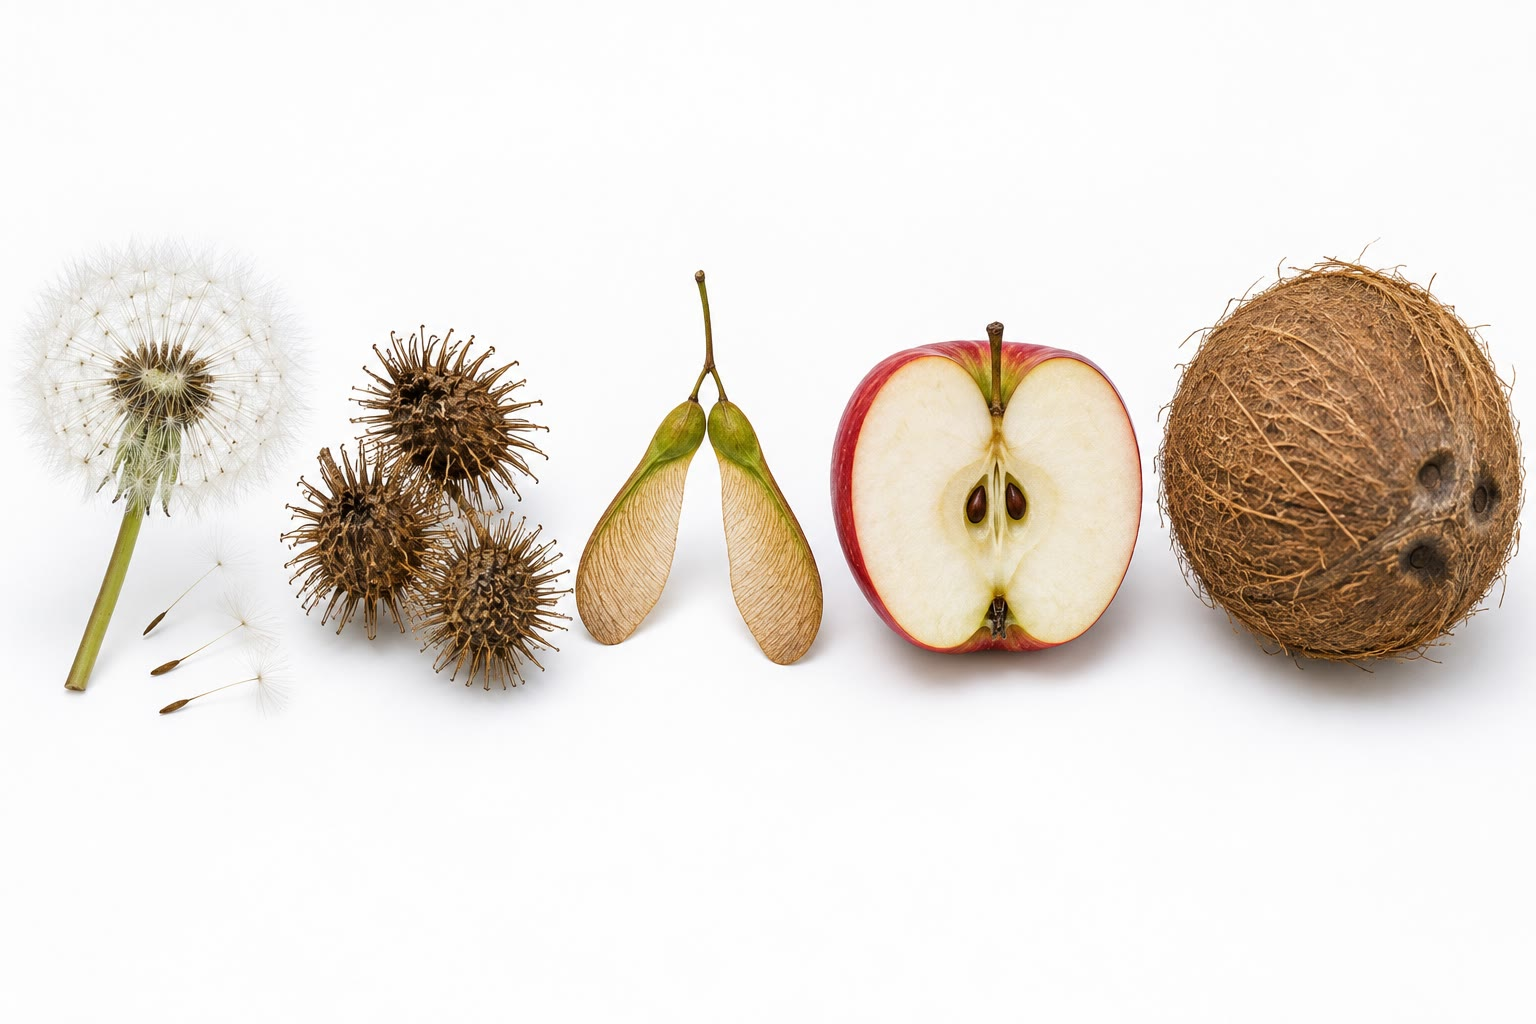
\includegraphics[width=0.62\linewidth]{images/book4/ai/b4-06-fruits-seeds.jpg}

{\small 为传播而设计的\omterm{def:b2:angiosperm-reproduction:seed}{果实}：冠毛（蒲公英）、
钩刺（牛蒡）、翅果（枫树）、供动物取食的果肉（苹果），以及
适于海上漂浮的外果皮（椰子）。}
\end{omfigure}

\begin{example}[传播距离]\label{ex:b2:angiosperm-reproduction:dispersal}
带冠毛的蒲公英瘦果以 \qty{0.3}{m/s} 的速度下降；
在 \qty{3}{m/s} 的风中，它从 \qty{0.3}{m} 高处可飞 \qty{3}{m}，
若遇上热气流，则可飞数百米。枫树的翅果自转下降，
自 \qty{15}{m} 高处以 \qty{1}{m/s} 的速度下降，可飞 \qty{45}{m}。一颗樱桃核被
鸟衔走，经二十分钟、以 \qty{10}{m/s} 的速度飞行后丢下，最远可达 \qty{12}{km}。橡树的橡子
若无松鸦搬运，便只落在树下。松鸦每次可搬运成千上万颗，
距离达一公里以上，并
会遗忘其中的十分之一。末次冰期之后重新迁入欧洲的橡树
每年向北迁移数百米，远快于橡子自行滚动的速度，
而推动它们迁移的正是鸟类。
\end{example}

\section{练习}

\begin{exercise}[$\star$]\label{exo:b2:angiosperm-reproduction:1}
说出花的四轮结构，以及\omterm{def:b2:angiosperm-reproduction:flower}{雄蕊}和\omterm{def:b2:angiosperm-reproduction:flower}{心皮}各自的组成部分，
并指出哪些部分属于\omterm{def:b2:meiosis-heredity:meiosis}{二倍体}\omterm{def:b2:plant-life-cycles:cycles}{孢子体}，哪些属于\omterm{def:b2:meiosis-heredity:meiosis}{单倍体}
\omterm{def:b2:plant-life-cycles:cycles}{配子体}？
\end{exercise}

\begin{exercise}[$\star$]\label{exo:b2:angiosperm-reproduction:2}
给出下列结构的倍性：\omterm{def:b2:plant-life-cycles:heterospory}{小孢子}、营养细胞、精子、
卵细胞、\omterm{prop:b2:angiosperm-reproduction:embryosac}{极核}、受精卵、\omterm{prop:b2:angiosperm-reproduction:double}{胚乳}、\omterm{def:b2:angiosperm-reproduction:seed}{种皮}、
果皮。
\end{exercise}

\begin{exercise}[$\star$]\label{exo:b2:angiosperm-reproduction:3}
列出风媒花的五个特征和蜂媒花的五个特征，
并各举一种植物为例。
\end{exercise}

\begin{exercise}[$\star$]\label{exo:b2:angiosperm-reproduction:4}
什么是\omterm{prop:b2:angiosperm-reproduction:double}{双受精}，两次融合各产生什么结构，
并说明为什么\omterm{prop:b2:angiosperm-reproduction:double}{胚乳}可被称为“按需定制”？
\end{exercise}

\begin{exercise}[$\star\star$]\label{exo:b2:angiosperm-reproduction:5}
玉米花丝长 \qty{25}{cm}，\omterm{thm:b2:angiosperm-reproduction:tube}{花粉管}生长
速度为 \qty{1.2}{cm/h}。授粉后需多长时间才能完成受精？
雄穗在第 0 天至第 7 天散粉，植株的花丝在
第 5 天至第 12 天抽出，每天抽出总数的八分之一；
花丝只在散粉期间才能接收\omterm{def:b2:plant-life-cycles:heterospory}{花粉}。被授粉的花丝占
总数的比例是多少？
\end{exercise}

\begin{exercise}[$\star\star$]\label{exo:b2:angiosperm-reproduction:6}
在\omterm{def:b2:plant-life-cycles:cycles}{配子体}\omterm{prop:b2:angiosperm-reproduction:selfing}{自交不亲和}的条件下，
杂交 $S_1S_2\times S_1S_2$、$S_1S_2\times
S_1S_3$、$S_1S_2\times S_3S_4$（雌蕊亲本列在前）中，相容\omterm{def:b2:plant-life-cycles:heterospory}{花粉}所占的比例各为多少？
求第二个杂交组合子代的\omterm{def:b2:meiosis-heredity:vocabulary}{基因型}。
\end{exercise}

\begin{exercise}[$\star\star$]\label{exo:b2:angiosperm-reproduction:7}
在一个含有 $n$ 个等频 $S$ \omterm{def:b2:meiosis-heredity:vocabulary}{等位基因}的种群中，
随机\omterm{def:b2:plant-life-cycles:heterospory}{花粉}中与某一给定植株相容的比例为多少？解释
由\omterm{def:b2:genome-diversification:mutation}{突变}产生的新 $S$ \omterm{def:b2:meiosis-heredity:vocabulary}{等位基因}为何会扩散，
并说明这对\omterm{def:b2:meiosis-heredity:vocabulary}{等位基因}数目有何预测。
\end{exercise}

\begin{exercise}[$\star\star$]\label{exo:b2:angiosperm-reproduction:8}
\omterm{def:b2:meiosis-heredity:vocabulary}{杂合} $Yy$（黄色\omterm{prop:b2:angiosperm-reproduction:double}{胚乳}为\omterm{def:b2:meiosis-heredity:vocabulary}{显性}）的玉米植株
自交。求其籽粒的\omterm{prop:b2:angiosperm-reproduction:double}{胚乳}\omterm{def:b2:meiosis-heredity:vocabulary}{基因型}及其比例，
注意两个\omterm{prop:b2:angiosperm-reproduction:embryosac}{极核}是相同的。
黄色籽粒所占的比例为多少？若改用
$yy$ 植株授粉，结果又如何？
\end{exercise}

\begin{exercise}[$\star\star$]\label{exo:b2:angiosperm-reproduction:9}
描述糊粉层实验，并说明它在以下几方面揭示了什么：
(a) 胚的作用，(b) 赤霉素的作用，(c)
淀粉酶合成的部位。为什么去胚的半粒籽粒是必不可少的
对照？
\end{exercise}

\begin{exercise}[$\star\star\star$]\label{exo:b2:angiosperm-reproduction:10}
从成本角度比较风媒与动物媒两种策略：风媒植物
每个\omterm{def:b2:plant-life-cycles:heterospory}{胚珠}产生 $10^{6}$ 粒\omterm{def:b2:plant-life-cycles:heterospory}{花粉}，每粒 \qty{1}{\micro g}；动物媒
植物每个\omterm{def:b2:plant-life-cycles:heterospory}{胚珠}产生 $10^{3}$ 粒\omterm{def:b2:plant-life-cycles:heterospory}{花粉}，每粒
\qty{1}{\micro g}，另加每朵花 \qty{5}{mg} 的\omterm{def:b2:angiosperm-reproduction:pollination}{花蜜}糖，
每朵花含十个\omterm{def:b2:plant-life-cycles:heterospory}{胚珠}。计算两种情况下每个\omterm{def:b2:plant-life-cycles:heterospory}{胚珠}的繁殖成本
（\omterm{def:b2:plant-life-cycles:heterospory}{花粉}与糖取相同的每克能量），并解释为何
风媒\omterm{def:b2:angiosperm-reproduction:pollination}{传粉}仍然存在。
\end{exercise}

\begin{exercise}[$\star\star\star$]\label{exo:b2:angiosperm-reproduction:11}
结合\cref{ex:b2:angiosperm-reproduction:dispersal}中的数据，
解释为何肉质\omterm{def:b2:angiosperm-reproduction:seed}{果实}对树木而言值得付出这一代价，尽管
动物消化果肉，并把大部分\omterm{def:b2:angiosperm-reproduction:seed}{种子}丢在无法
萌发的地方。
\end{exercise}

\begin{exercise}[$\star\star\star$]\label{exo:b2:angiosperm-reproduction:12}
“闭合\omterm{def:b2:angiosperm-reproduction:flower}{心皮}是被子植物统治
陆地的原因。”讨论：\omterm{def:b2:plant-life-cycles:heterospory}{胚珠}被包裹后能带来什么
（\omterm{def:b2:plant-life-cycles:heterospory}{花粉}的选择、不亲和性、\omterm{def:b2:angiosperm-reproduction:seed}{果实}），以及它付出的代价。
\end{exercise}

\section{问题：一座果园与一块田地}

\begin{problem}[{周末问题——苹果园的授粉规划（依据自交不亲和性），
以及玉米田的受精与产量（由其产生的花粉计算），
最后归结为果园的坐果率，
以及田地的籽粒数}]
\label{pb:b2:angiosperm-reproduction:1}
苹果为\omterm{def:b2:plant-life-cycles:cycles}{配子体}型\omterm{prop:b2:angiosperm-reproduction:selfing}{自交不亲和}。一座果园有三个品种：
A（$S_1S_2$）、B（$S_1S_3$）、C（$S_3S_4$）。一朵花有五个\omterm{def:b2:angiosperm-reproduction:flower}{心皮}，
每个\omterm{def:b2:angiosperm-reproduction:flower}{心皮}含两枚\omterm{def:b2:plant-life-cycles:heterospory}{胚珠}，结\omterm{def:b2:angiosperm-reproduction:seed}{种子}不足五粒的\omterm{def:b2:angiosperm-reproduction:seed}{果实}
会被树木脱落。一次蜜蜂访花在\omterm{def:b2:angiosperm-reproduction:flower}{柱头}上留下\num{100}~
粒\omterm{def:b2:plant-life-cycles:heterospory}{花粉}；每粒相容\omterm{def:b2:plant-life-cycles:heterospory}{花粉}有 $0.1$ 的概率使
一枚尚未被占用的\omterm{def:b2:plant-life-cycles:heterospory}{胚珠}受精。一棵树着生\num{5000}朵花
满产需要\num{250}个\omterm{def:b2:angiosperm-reproduction:seed}{果实}。玉米的雄穗散粉
$10^{7}$ 粒，历时\num{7}~天；田间每平方米
种植\num{8}株；每株一穗，穗上\num{600}条花丝；
每条花丝迎受落粉的面积为\qty{1e-4}{m^2}；\omterm{def:b2:plant-life-cycles:heterospory}{花粉}沉降速度为
\qty{0.25}{m/s}；每粒籽粒含\omterm{prop:b2:angiosperm-reproduction:double}{胚乳}\qty{0.3}{g}。

\medskip
\noindent\textbf{第一部分——相容性。}
\begin{enumerate}
  \item 对 A 植株雌蕊上各品种的\omterm{def:b2:plant-life-cycles:heterospory}{花粉}，
        给出相容比例 $f$。
  \item 对 B 与 C 的雌蕊，同样计算。
  \item 一只来自 B 树的蜜蜂在 A 的\omterm{def:b2:angiosperm-reproduction:flower}{柱头}上留下 100 粒\omterm{def:b2:plant-life-cycles:heterospory}{花粉}：
        有多少粒相容，
        预期有多少\omterm{def:b2:plant-life-cycles:heterospory}{胚珠}受精（忽略饱和）？
  \item 来自 C 树的蜜蜂，以及来自另一株 A 的蜜蜂，同样计算。
  \item 哪些\omterm{def:b2:angiosperm-reproduction:seed}{果实}会被保留？单独种植
        A 品种的果园有何风险？
  \item A 树成片，外围为 C 树；A 的蜜蜂访花中，一半来自 C。
        若每朵花接受一次访花，
        则 A 花的坐果比例为多少，每棵树结多少\omterm{def:b2:angiosperm-reproduction:seed}{果实}？
        产量是否满额？
  \item 果园为何要间种开花持续数周的海棠，
        其 $S$ \omterm{def:b2:meiosis-heredity:vocabulary}{等位基因}为何必须检验？
\end{enumerate}

\medskip
\noindent\textbf{第二部分——玉米田上的\omterm{def:b2:plant-life-cycles:heterospory}{花粉}。}
\begin{enumerate}[resume]
  \item 计算每平方米田地每秒释放的\omterm{def:b2:plant-life-cycles:heterospory}{花粉}数，
        取七天的平均值。
  \item 稳态时，沉降\omterm{def:b2:plant-life-cycles:heterospory}{花粉}的通量等于释放速率。
        计算空气中的\omterm{def:b2:plant-life-cycles:heterospory}{花粉}浓度
        （粒/立方米）。
  \item 计算每秒落在一条花丝上的\omterm{prop:b2:angiosperm-reproduction:pollen}{花粉粒}数，
        以及第一粒\omterm{def:b2:plant-life-cycles:heterospory}{花粉}的平均等待时间。
  \item 一条花丝一天接收多少粒\omterm{def:b2:plant-life-cycles:heterospory}{花粉}？为何只有
        第一粒有用？
  \item 一条\qty{20}{cm}长的花丝被授粉，\omterm{thm:b2:angiosperm-reproduction:tube}{花粉管}以
        \qty{1}{cm/h}的速度生长。\omterm{def:b2:plant-life-cycles:heterospory}{胚珠}何时受精？
  \item 干旱使花丝抽出推迟五天，而雄穗按时散粉。
        以七天的散粉期为依据，
        估算花丝所接收的\omterm{def:b2:plant-life-cycles:heterospory}{花粉}占整个\omterm{def:b2:plant-life-cycles:heterospory}{花粉}季的比例，
        及其对产量的影响。
\end{enumerate}

\medskip
\noindent\textbf{第三部分——\omterm{prop:b2:angiosperm-reproduction:double}{双受精}与籽粒。}
该田地种植黄色\omterm{prop:b2:angiosperm-reproduction:double}{胚乳}品种（$Y$，\omterm{def:b2:meiosis-heredity:vocabulary}{显性}），
旁边是白色（$yy$）的田地；风从白色田地吹来。
\begin{enumerate}[resume]
  \item 给出籽粒胚与\omterm{prop:b2:angiosperm-reproduction:double}{胚乳}的\omterm{def:b2:meiosis-heredity:vocabulary}{基因型}，该籽粒
        来自 $YY$ 植株，由 $yy$ \omterm{def:b2:plant-life-cycles:heterospory}{花粉}受精。
  \item 籽粒是黄色还是白色？解释术语“\omterm{def:b2:plant-life-cycles:heterospory}{花粉}直感”。
  \item 一株 $Yy$ 植株由 $yy$ \omterm{def:b2:plant-life-cycles:heterospory}{花粉}授粉：
        给出\omterm{prop:b2:angiosperm-reproduction:double}{胚乳}的\omterm{def:b2:meiosis-heredity:vocabulary}{基因型}及其频率。
  \item \omterm{prop:b2:angiosperm-reproduction:double}{胚乳}含两个母本染色体组和一个父本染色体组。
        某基因具有剂量效应，每个拷贝产生 10~单位色素：
        籽粒 $YYy$、$Yyy$ 和 $yyY$ 各带有何种色素：
        （假设父本剂量为两份）携带多少？其中哪些
        实际上可以存在？
  \item 为何人类食用的是\omterm{prop:b2:angiosperm-reproduction:double}{胚乳}而非胚，
        以及\omterm{prop:b2:angiosperm-reproduction:double}{胚乳}占籽粒质量的比例是多少，若胚重
        \qty{0.03}{g}。
  \item 为何\omterm{prop:b2:angiosperm-reproduction:double}{胚乳}的“按需定制”式供养是一种优势，
        相较于裸子植物的供养方式？
\end{enumerate}

\medskip
\noindent\textbf{第四部分——产量。}
\begin{enumerate}[resume]
  \item 若 \qty{90}{\%} 的花丝受精，计算每穗、每株
        及每平方米的籽粒数，以及每平方米的\omterm{prop:b2:angiosperm-reproduction:double}{胚乳}
        质量。
  \item 换算为每公顷吨数。
  \item 作物每平方米每季固定 \qty{1.2}{kg} 碳，其中一半
        进入收获的籽粒。请检验与第 20 题
        中的质量是否一致（\omterm{prop:b2:angiosperm-reproduction:double}{胚乳}含碳
        \qty{45}{\%}）。
  \item 田间每收获一粒籽粒，
        散落了多少粒\omterm{def:b2:plant-life-cycles:heterospory}{花粉}？
  \item 解释为何花园中孤立的一株玉米结出的穗
        籽粒不饱满。
  \item 给出结果：A 区的坐果率，以及田地的
        产量，以每平方米籽粒数和每
        公顷吨数表示。
\end{enumerate}
\end{problem}
